\chapter{2. Background}

The aim of this chapter is to critically review the literature relevant to the study of tilting three wheelers and their control strategies.

\section{Active and Passive Tilting}

The dynamics of a tilting PEV are quite different from a conventional car. Indeed, due to the narrow track of these type of vehicles, and according to the position of their \textbf{center of gravity}, their dynamics on turning may be closer to the dynamics of two-wheeler vehicles such as motorcycles.

\begin{marginfigure}
	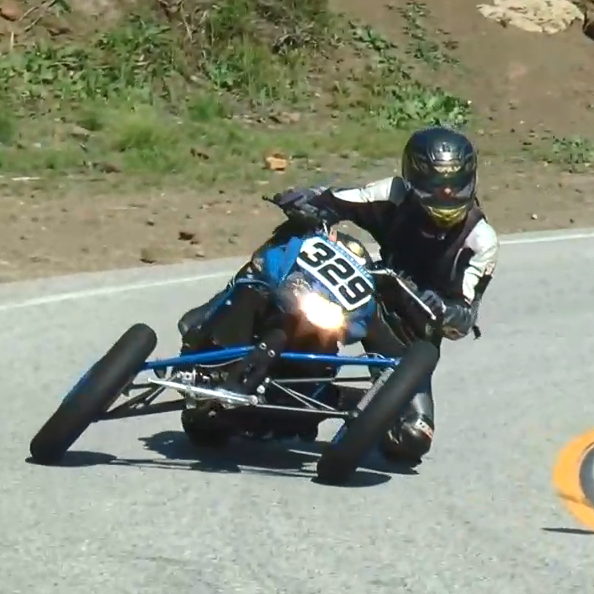
\includegraphics[width=1.0\linewidth]{figs/02/passive}
	\caption{Passive tilting system from \textit{Tilting Motor Works}}
\end{marginfigure}
\begin{marginfigure}
	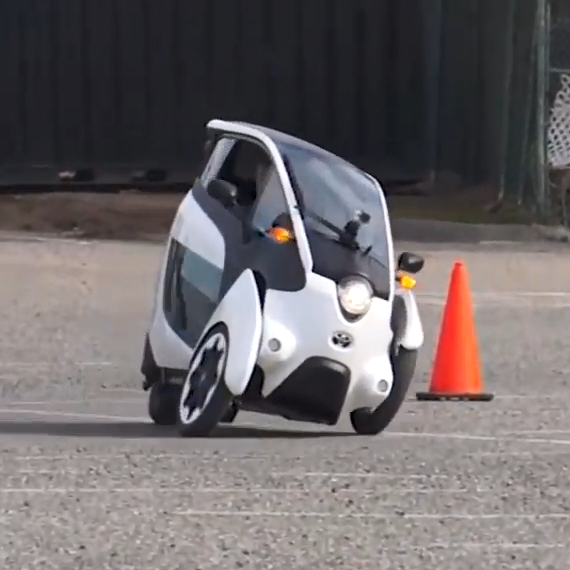
\includegraphics[width=1.0\linewidth]{figs/02/active}
	\caption{Active tilting system from the \textit{Toyota i-ROAD concept car}}
\end{marginfigure}

Thus, some of these vehicles have to tilt when turning to compensate for the effect of lateral acceleration and remain in balance. In the case of a motorcycle, it is the driver who causes the lateral movement of the motorcycle (\textbf{passive tilting}), whereas for heavy and bulky vehicles, the inclination must be automatic (\textbf{active tilting}). 

The main drawback with a passive tilting system is the necessity of a \textbf{locking mechanism to avoid the leaning} of the vehicle when standing. On the contrary, an active system does not need a locking mechanism, since is an actuated mechanism. In addition, the ability to control the leaning can facilitate users to get on the vehicle by leaning to one side and returning to the vertical position to start the ride.

Theferore, this problem of \textbf{stability in the curves} is a major technological challenge for these narrow vehicles. Some manufacturers have solved the difficulty by lowering the center of gravity of the vehicle to a minimum (see Tango\cite{tango} or Twizy\cite{twizy}), for example by placing the batteries very low if it is an electric vehicle. 

In the case of narrow active tilting vehicles, different actuating and control strategies have been studied in the industry, which are presented below (DTC, STC or SDTC).

\section{Narrow Three-Wheeled Vehicles}

In this section narrow tilting vehicles with three wheels are presented. In order to easily identify the different types, the following notation is adopted: \textbf{[ nF, tT, pP, S ]} with n the number of front wheels, t the number of tilting wheels, p the number of passengers and S the maximum speed in $Km / h$.

\begin{itemize}
	\begin{itemize}
	\item \textbf{GM Lean Machine}\cite{leanmachine} (1F, 1T, 1P, 125) was developed by Frank Winchell of General Motors in the early 1980's. The lateral stability of the vehicle had to be ensured by the driver, through a pedal that controlled the tilt. 

	\item \textbf{Mercedes Life Jet F300}\cite{f300} (2F, 3T, 2P, 210) was introduced in 1997 by Mercedes-Benz at the Frankfurt Motor Show. The tilt was automated through hydraulic actuators. 
	
	\item \textbf{CLEVER}\cite{clever} (1F, 1T, 2P, 80), was developed at the University of Bath (UK) in collaboration with BMW. The inclination of the front module of the vehicle is possible thanks to the hydraulic actuators linking the cab to the non-tilting rear part. The first prototypes were built in 2006, but the transient behavior of this vehicle did not always guarantee lateral stability.
	
	\item \textbf{Carver One}\cite{ClassAvec04} (1F, 1T, 2P, 185), a three-wheel tilting vehicle, born from a first aerodynamic concept. The Carver One is equipped with an automotive power unit and therefore with a wide non-tilting rear axle. The dynamics of the vehicle are based on the patented 'Dynamic Vehicle Control' technology, which is said to ensure vehicle stability by tilting the vehicle. 
	
	\item \textbf{Piaggio MP3 Hybrid 300IE}\cite{piaggio} (2F, 3T, 1P, 145), is a three-wheeled scooter with a parallel "hybrid" propulsion, based on a 125 cc engine and a 3.4 hp electric motor. Like a traditional scooter, this vehicle is tilted directly by the driver. 
		\end{itemize}
\end{itemize}

Paying attention to more lightweight vehicles (bike-like):
	
\begin{itemize}
	\begin{itemize}
	\item \textbf{Veleon}\cite{veleon} (2F, 3T, 1P, 25) both cargo and driver lean into the curve, helping to whoosh cars and other obstacles, including tight corners at high speed. The mode can be deactivated by pressing a button and the bicycle stays in vertical position.
	
	\item \textbf{Trego}\cite{trego} (2F, 3T, 1P, 25) is a successful fusion of a cargo bike and a folding bike, a modular separable tricycle. Combines a rear wheel to two front wheels, that are connected by an L structure, being extremely useful for transporting bulky items.
	
	\item \textbf{Kaylad-e}\cite{kaylad} (2F, 3T, 1P, 25) is a tilting trike concept with a 250-W electric motor and a lithium battery. The concept also includes a secure luggage holder or and optional heavy-duty container that can be mounted on the front of the bicycle.

	\item \textbf{Carqon}\cite{carqon} (2F, 3T, 1P, 30) has a patented carving mechanism underneath the frame and is equipped with a high torque motor for maximum torque and performance. It is similar to riding a normal bicycle where the driver uses his/her body to control the steering more than actually the turning of the handlebar.
}
	\\[5pt]
	\end{itemize}
\end{itemize}

\begin{marginfigure}
	\caption{Tilting Vehicles}
\end{marginfigure}

\begin{figure*}[h]
		\minipage{0.32\textwidth}
		  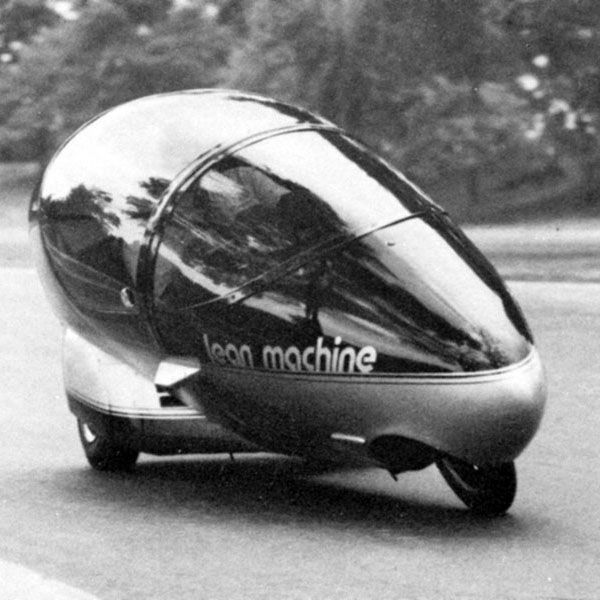
\includegraphics[width=1.0\linewidth]{figs/02/gmlean}
		  \captionof{a)}{ GM Lean Machine}
		\endminipage\hfill
		\minipage{0.32\textwidth}
		  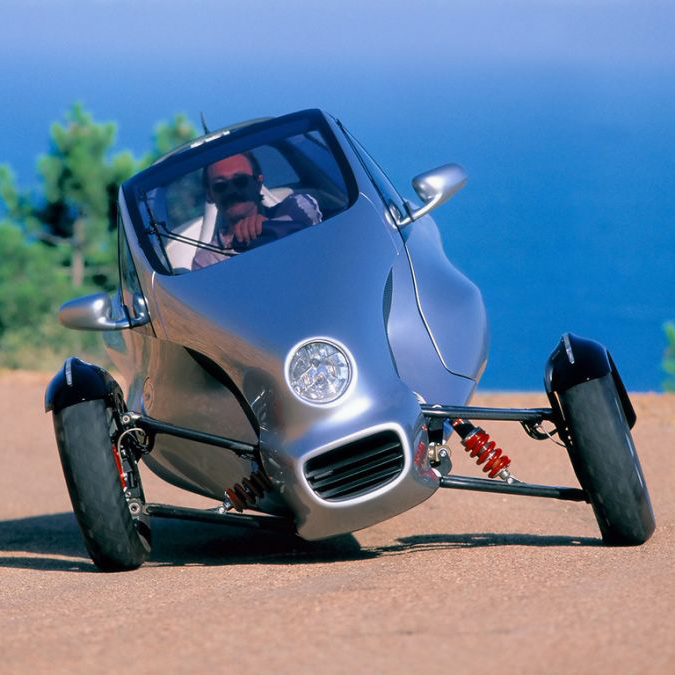
\includegraphics[width=1.0\linewidth]{figs/02/mercedes}
		  \captionof{b)}{ Mercedes Life Jet F300}
		\endminipage\hfill
		\minipage{0.32\textwidth}%
		  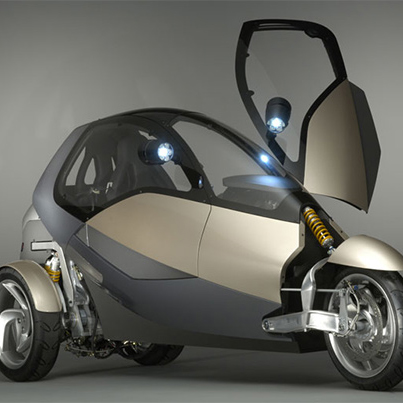
\includegraphics[width=1.0\linewidth]{figs/02/clever}
		  \captionof{c)}{ CLEVER}
		\endminipage
		\\[0pt]
\end{figure*}
		  
\begin{figure*}[h]
		\minipage{0.32\textwidth}
		  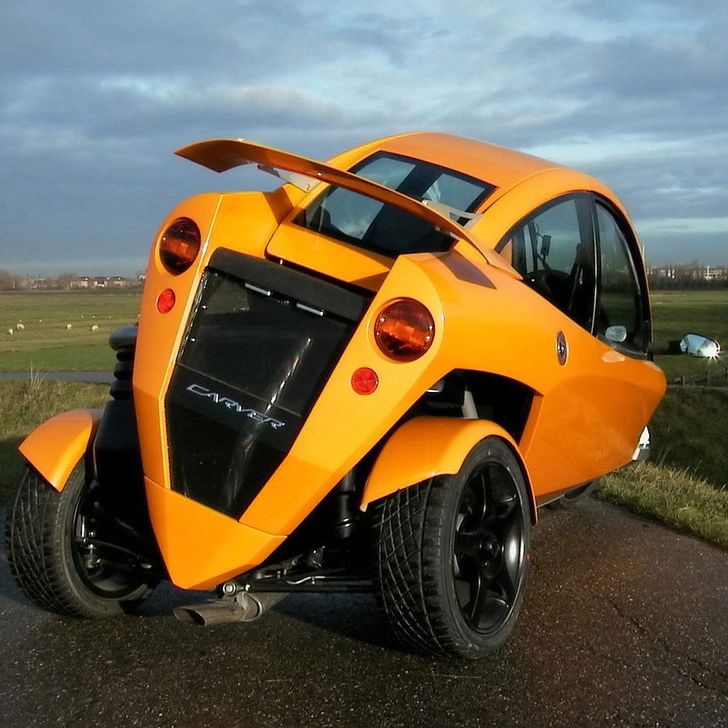
\includegraphics[width=1.0\linewidth]{figs/02/carver}
		  \captionof{d)}{ Carver One}
		\endminipage\hfill
		\minipage{0.32\textwidth}
		  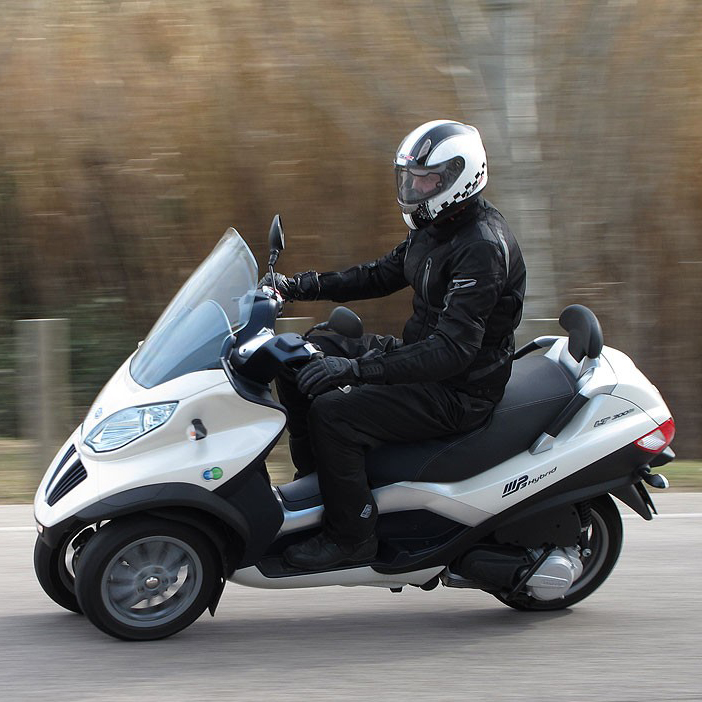
\includegraphics[width=1.0\linewidth]{figs/02/piaggio}
		  \captionof{e)}{ Piaggio MP3 Hybrid 300IE}
		\endminipage\hfill
		\minipage{0.32\textwidth}%
		  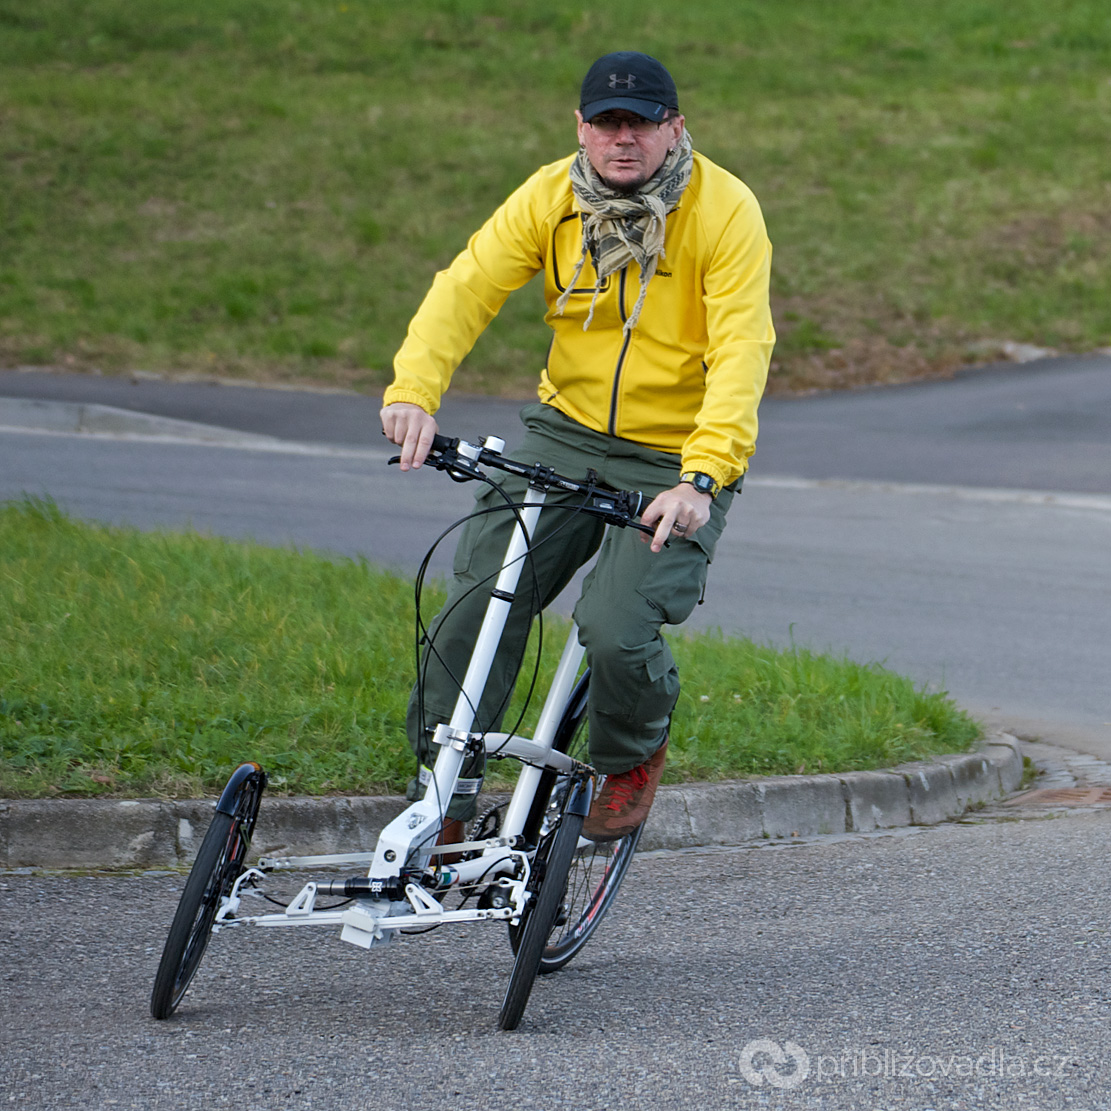
\includegraphics[width=1.0\linewidth]{figs/02/veleon}
		  \captionof{f)}{ Veleon}
		\endminipage
		\\[0pt]
\end{figure*}

\begin{figure*}[!h]
		\minipage{0.32\textwidth}
		  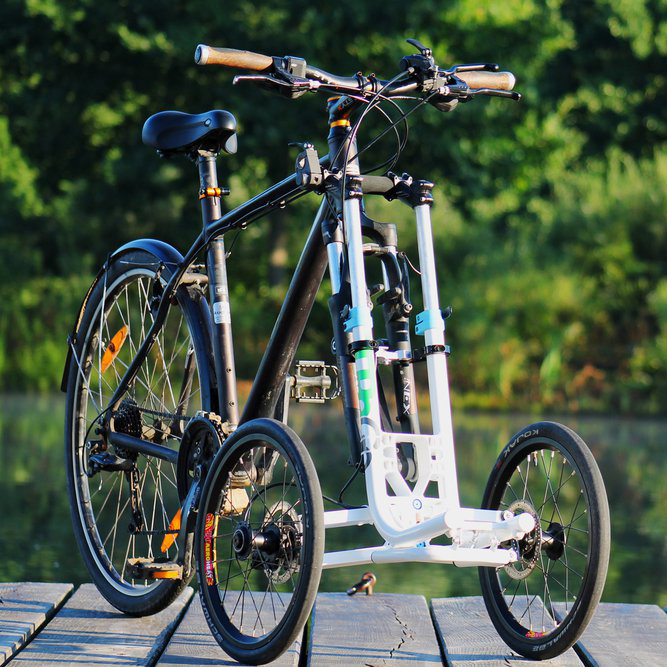
\includegraphics[width=1.0\linewidth]{figs/02/trego}
		  \captionof{g)}{ Trego}
		\endminipage\hfill
		\minipage{0.32\textwidth}
		  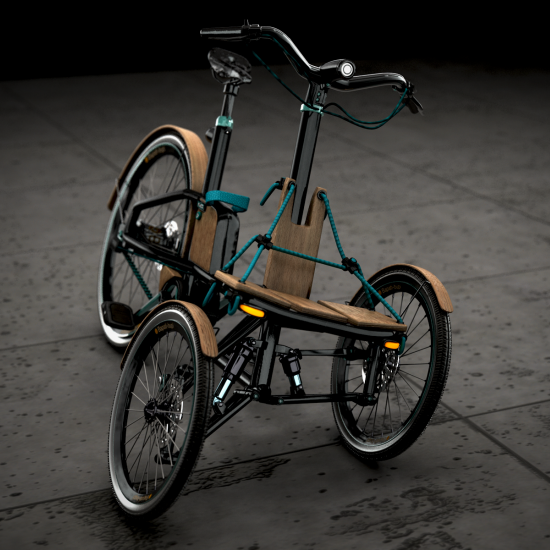
\includegraphics[width=1.0\linewidth]{figs/02/kaylad}
		  \captionof{h)}{ Kaylad-e}
		\endminipage\hfill
		\minipage{0.32\textwidth}%
		  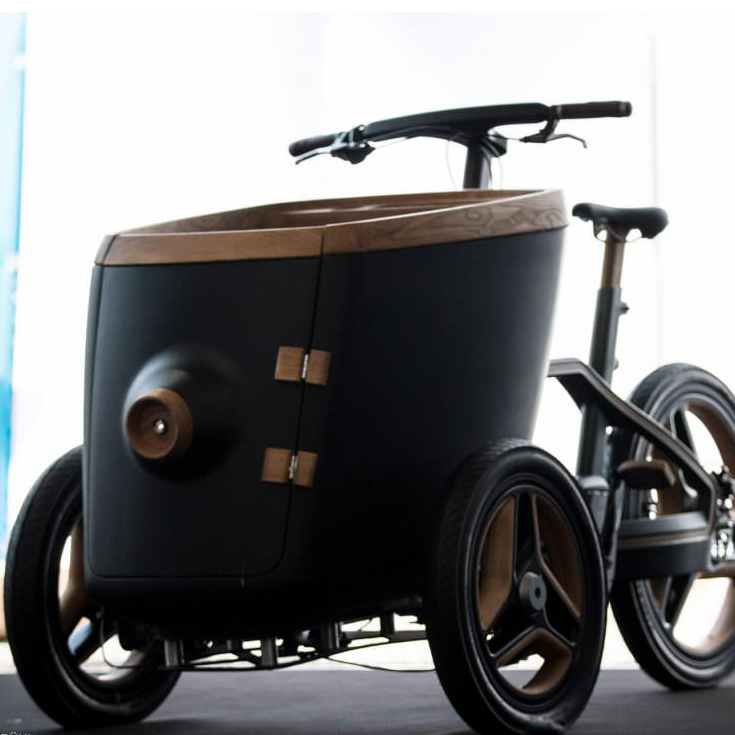
\includegraphics[width=1.0\linewidth]{figs/02/carqon}
		  \captionof{i)}{ Carqon}
		\endminipage
\end{figure*}

\newpage

\section{Tilt-Actuating Architectures}
\subsection{Direct Tilt Control (DTC)}

The inclination is achieved by means of actuators mounted directly on the longitudinal axis of the vehicle, \textbf{providing a torque} ($M_t$) to tilt the whole vehicle or some parts of it. It is the most used system on narrow tilting vehicles and the simplest active system to implement.

\begin{marginfigure}
	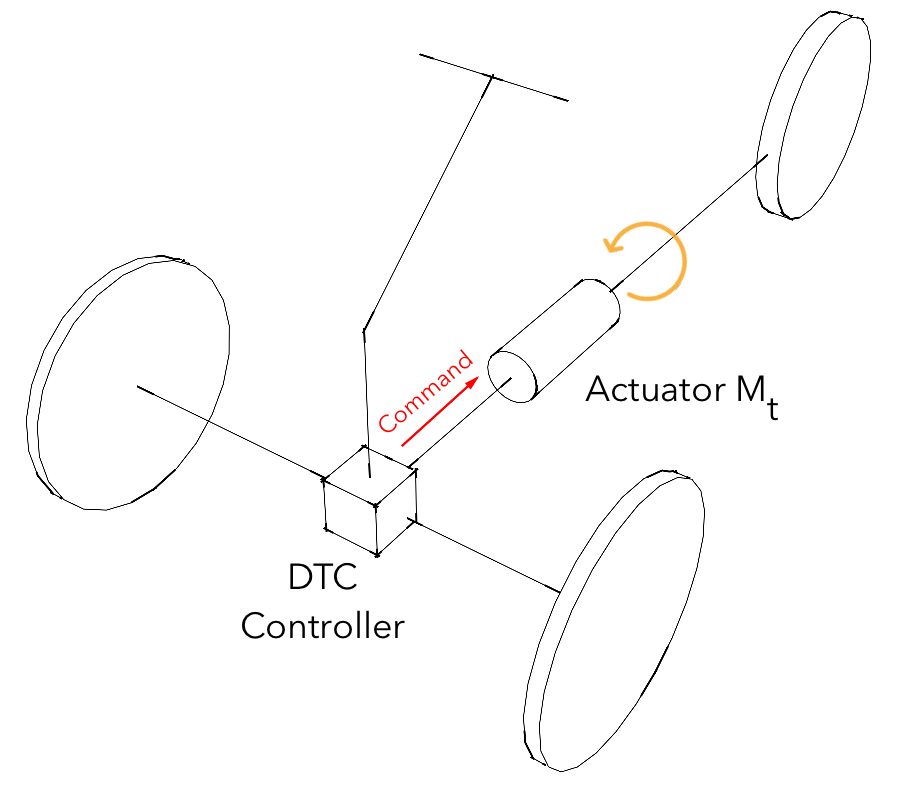
\includegraphics[width=1.0\linewidth]{figs/02/dtc_diagram}
	\caption{DTC system schematic}
\end{marginfigure}

In a turn, the lateral acceleration is proportional to the longitudinal velocity, as is demonstrated in the next chapter. Therefore, for the same steering angle, the lateral acceleration is higher at high speed. As a result, the \textbf{torque $M_t$ required is greater at high speed} since it must ensure the desired inclination in the opposite direction to that of the lateral acceleration. 

It is at high speed that there is a greater risk of \textbf{saturation of the actuator}. It should be noted that if the DTC system only acts from the measurement of the measured acceleration, this may cause an unpleasant feeling in the passengers. When driving a motorcycle, the rider tilts the vehicle simultaneously with the taking of the turn, so that the perceived acceleration remains virtually zero, even in transient situations.

\subsection{Steering Tilt Control (STC)}

These systems control the steering angle of the wheels. The steering angle ($\delta_{driv}$) applied by the driver is modulated by the STC system ($\delta_c$) to control the tilt angle using countersteering. This strategy is inspired by the action of a bicycle or motorcycle rider, but is seldom used by manufacturers, since it is based on a \textbf{steer-by-wire} system, which is still prohibited to commercialize for safety standards reasons.

\begin{marginfigure}
	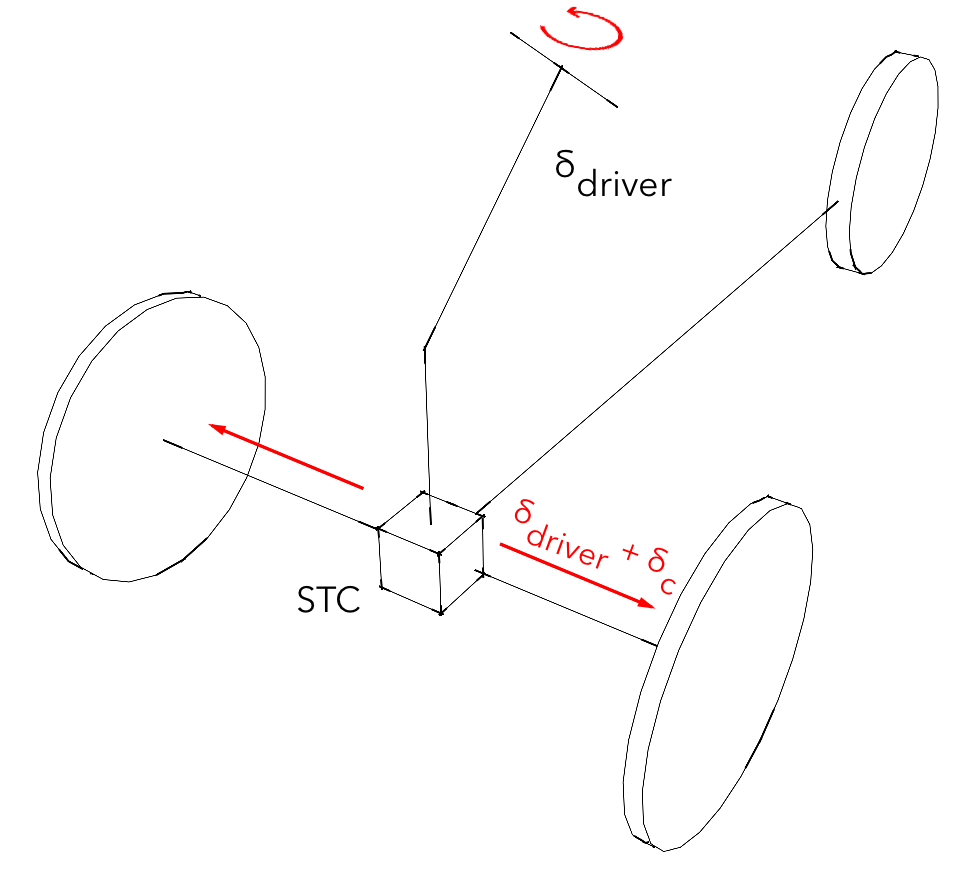
\includegraphics[width=1.0\linewidth]{figs/02/stc_diagram}
	\caption{STC system schematic}
\end{marginfigure}

STC systems are not well suited for \textbf{low longitudinal speeds}, demanding a large counter-steering to tilt the vehicle, which deviates it significantly from its trajectory. In contrast, the STC system is more efficient than the DTC at high speed, as a large torque is required by the DTC (due to the delay in the DTC tilting torque).
\newpage

\subsection{Comparison between DTC and STC}

Let us compare both tilting systems by looking to the forces actuating in each case. The vehicle is traveling in an straight line at a constant velocity $V$, when a right turn comes.


	
\begin{itemize}
	\begin{itemize}
	\item DTC: the driver will turn the steering wheel to the right (Figure \ref{dtc}), producing a lateral acceleration in the inner direction of the curve( do not confuse it with the inertial force which pushes the vehicle outwards the curve). Due to the possibility of tilting, the vehicle will tend to lean to the left, but in this moment the DTC torque $M_t$ will correctly lean it to the right. In this simple case it is clear the delay between the lateral acceleration and the torque $M_t$.
	\begin{figure}[h]
		\minipage{0.32\textwidth}
		  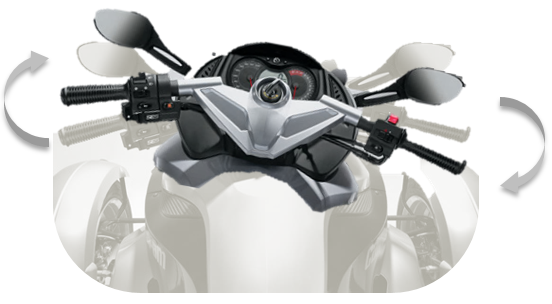
\includegraphics[width=1.0\linewidth]{figs/02/dtc_1}
		\endminipage\hfill
		\minipage{0.32\textwidth}
		  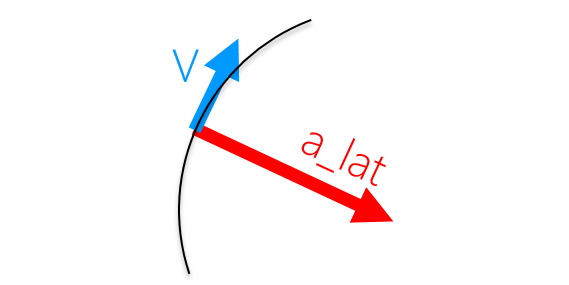
\includegraphics[width=1.2\linewidth]{figs/02/dtc_2}
		\endminipage\hfill
		\minipage{0.32\textwidth}%
		  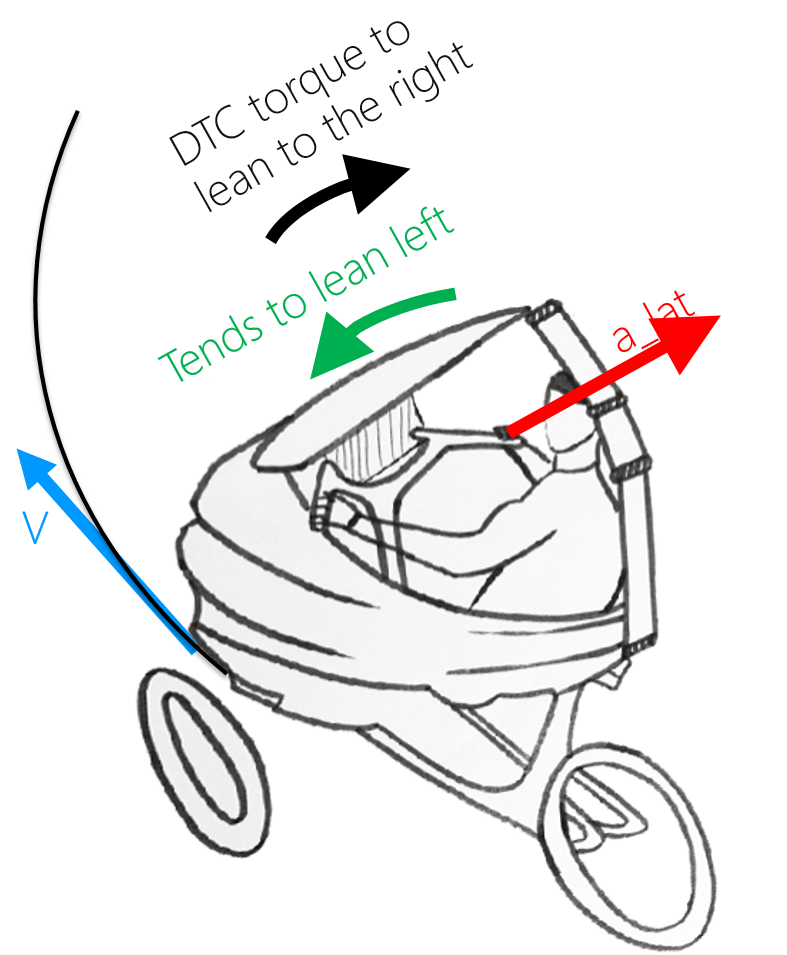
\includegraphics[width=1.0\linewidth]{figs/02/dtc_3}
		\endminipage
		\label{dtc}
		\caption{Direct Tilt Control \protect\\ a) Steering input from the driver \protect\\ b) DTC force diagram in a right turn \protect\\ c) DTC tilting torque input}
		\\[1pt]
	\end{figure}
	\item STC: the STC steer-by-wire system will slightly turn the steering wheel to the left (Figure \ref{stc}), producing a lateral acceleration in the outer direction of the curve. Due to the possibility of tilting, the vehicle will correctly lean to the right. By using the countersteering, the vehicle easyly leans to the appropiate side, but the desired path of the user is not perfectly followed.
	\begin{figure}[h]
		\minipage{0.32\textwidth}
		  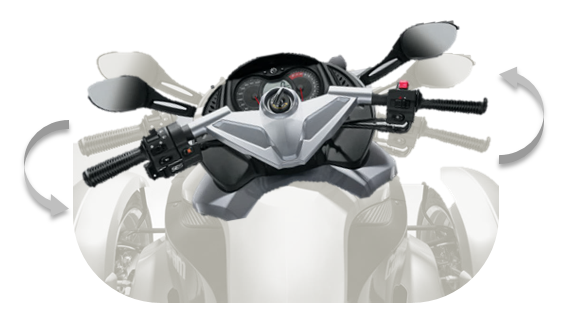
\includegraphics[width=1.0\linewidth]{figs/02/stc_1}
		\endminipage\hfill
		\minipage{0.32\textwidth}
		  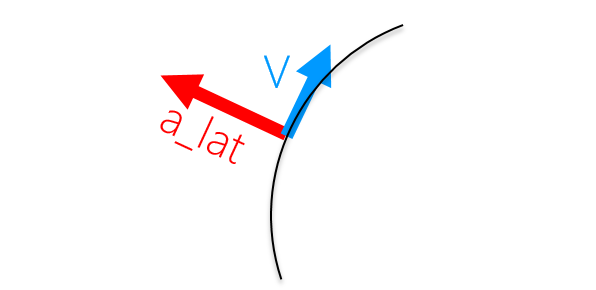
\includegraphics[width=1.2\linewidth]{figs/02/stc_2}
		\endminipage\hfill
		\minipage{0.32\textwidth}%
		  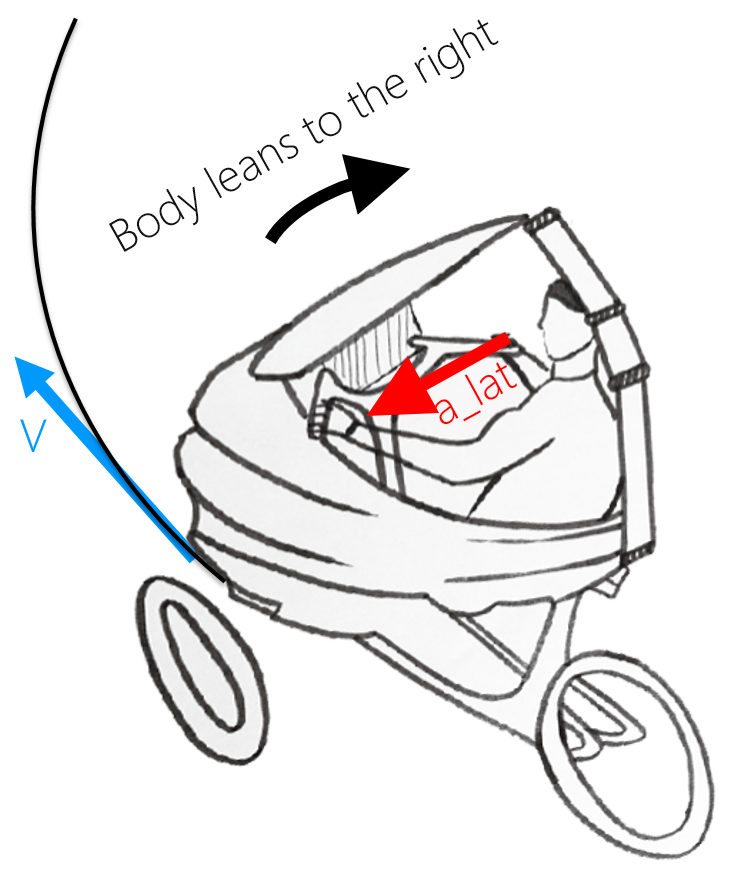
\includegraphics[width=1.0\linewidth]{figs/02/stc_3}
		\endminipage
		\caption{Steering Tilt Control: \protect\\a) Steering input from the actuator \protect\\b) STC force diagram in a right turn \protect\\c) STC tilts automatically in a right turn}
		\label{stc}
	\end{figure}
	\end{itemize}
\end{itemize}
\newpage
In order to give an overall view, the table \ref{dtc_vs_stc} summarizes the characteristics of the two systems DTC and STC.
\begin{table*}[h]
\centering
\caption{DTC vs STC comparison table}
\label{dtc_vs_stc}
	\begin{tabular}{l|c|c|}
	           & \textbf{DTC}                                   & \textbf{STC}                  \\
	\hline        
	\textbf{Lean by}    & Roll actuator                         & Countersteering                 \\
	\textbf{Stability}  & Always stable                         & Unstable at low speeds          \\
	\textbf{High Speed} & Deal with high lateral acceleration   & Small adjustments               \\
	\textbf{Low Speed}  & Good behaviour at low speeds: $M_t$ \Uparrow & Large and frecuent steer inputs $\delta_c$ \Uparrow
	\end{tabular}
	\\[20pt]
\end{table*}

\subsection{SDTC hybrid solution}
To take advantage of both strategies and their complementary efficiencies according to speed, recent work has focused on the so-called SDTC hybrid solution for vehicles with both a tilt actuator and a steer-by-wire system. The first solutions are monovariable, meaning that a single control input is active at a time, with switching from one system to the other as a function of the speed. 

The STC systems are generally implemented from a threshold speed of approximately $V=40 Km/h$ while the DTC systems are active below that speed. Switching from one system to another by switching is complicated due to the fact that the control signals act as antagonist in transient phases\cite{doi:10.1080/00423119708969321},\cite{hibbard1996twenty}.
\begin{itemize}
	\begin{itemize}
	\item In transient, the STC system causes a counter-steering, and the created lateral acceleration created serves for the inclination of the vehicle. Switching from STC to DTC, the DTC command will seek to tilt the vehicle in the opposite direction to the perceived lateral acceleration, hence in the wrong direction. The two control signals are conflicting or antagonistic in this case.

	\item Switching from DTC to STC, the control signals are not conflicting, but the tilt torque DTC $M_t$ abruptly cancels out as the vehicle starts to tilt. This interruption creates a discontinuity and peaks in the signals.
	\end{itemize}
\end{itemize}

\newpage

\section{Vehicle Model}
Modeling is a key step in the study and control of systems. Depending on the use to be made (embedded model, design model, simulation model...), different levels of complexity can be envisaged.

\subsection{Models Used in the Literature}
The study and development of narrow vehicles only began recently, due to the congestion problems of road traffic and the increase in pollution. The problem of narrow and tilting vehicles is therefore recent, and few research teams have worked on this subject. The \textbf{narrow tilting vehicle models} will be reviewed in this section, explaining their advantages and limitations. 

Researchers at \textbf{California University} were among the first to take an interest in this matter. In Hibbard R. \textit{et al.}, (1996)\cite[-4.5cm]{hibbard1996twenty} and So S. \textit{et al.}, (1997a)\cite[-1.7cm]{doi:10.1080/00423119708969321}, the authors consider only the dynamics of the angle of inclination $\theta$, and the model used for the simulation was reduced to the transfer function between the input $M_t$ and $\theta$. 

A more detailed linearized simulation model at small angles, with longitudinal dynamics, was used in later work (So S. \textit{et al.}, 1997b)\cite[-1.7cm]{doi:10.1504/IJVD.1997.062071}.

In the UK, at the \textbf{University of Bath}, the researchers worked on the CLEVER project. In his thesis\cite[-0.3cm]{bath24682}, J. Berote focused on the vehicle modeling, developing a 5 degree of freedom (dof) multi-body model, that included dynamics of hydraulic actuators, which was then incorporated into the SimMechanics software to obtain a validation model. 

Previously, they used a PID controller (J. Berote \textit{et al.}, 2008)\cite[-1cm]{bath15090}, that did not require any model. For such a purpose, the authors considered approximate relations between the steering angle and the lateral acceleration, and between the steering angle and the angle of inclination. 
\\
\begin{figure}[h!]
	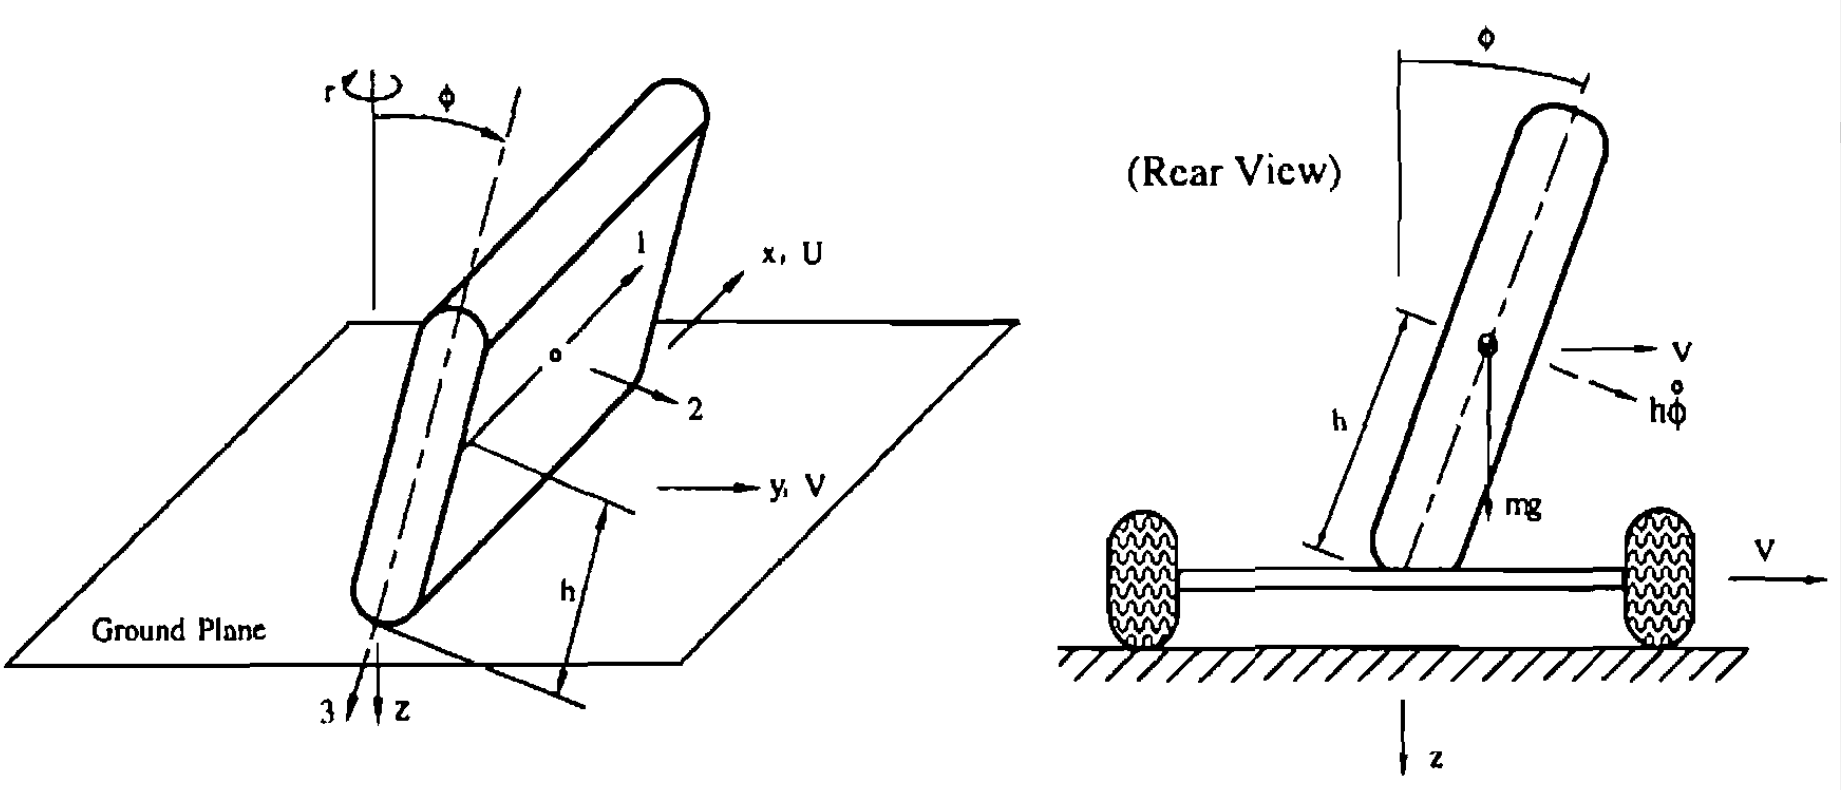
\includegraphics[width=1.0\linewidth]{figs/02/literature_model}
	\caption{Literature model: Inverted pendulum simple model for tilting vehicles }
	\label{literature}
	\\[-3cm]
\end{figure}

\newpage

At the \textbf{University of Minneapolis} in Minnesota, a prototype recliner was built, and several advances were made. In the article R. Rajamani \textit{et al.}, (2003)\cite[0cm]{doi:10.1076/mcmd.9.2.209.16521} the authors focus on modeling the vehicle. They neglect the longitudinal dynamics, but take into account the gyroscopic moments of the wheels and the tilting moment. 

Their synthesis model for the design of the control law, also used for simulation, was later simplified and a linearized model of equation (Piyabongkran D. \textit{et al.} 2004\cite{piyabongkarn2004active}, Kidane S. \textit{et al.}, 2010\cite{5356230}, Kidane S. \textit{et al.}, 2008\cite{doi:10.1080/00423110701352987}}).



%In France, at the \textbf{Ecole des Mines de Nantes}, L. Mourad et al.
%\newpage
\subsection{Bicycle Model}

The lateral control of the tilting vehicles is the object of this study. The so-called \textbf{bicycle model} has been chosen to be considered as a conceptual model which aggregates the 2 front wheels in one wheel, and only one rear wheel. Wheel torques are also simplified. They are implicitly replaced by the steering angle. 

This model has been built from the 4 dof model presented in the article of R. Rajamani \textit{et al.}, (2003)$^{19}$, which considers the longitudinal speed as a parameter of the model and not as a state variable.

The model obtained takes into account the longitudinal dynamics relating to the speed, as well as the lateral dynamics including the inclination. Figures \ref{xy} and \ref{yz} respectively show the views in the horizontal ($XY$) and vertical ($YZ$) planes of the vehicle. 

The quantities and notations used below are defined in the 'Notations' section at the beginning of the thesis. Let us define the following coordinate systems: 
\begin{enumerate}
\item The absolute coordinate system $R$=($X$, $Y$, $Z$) fixed to the ground, the axes $X$ and $Y$ are on the ground while the $Z$ is the vertical axis. 

\item The vehicle coordinate system $r$=($x$, $y$, $z$) is linked to the vehicle. Its origin is the point G (center of gravity), the axis $x$ is parallel to the longitudinal axis of the vehicle, the axis $z$ is parallel to the axis $Z$ and the axis $y$ is such that the planes $xy$ and $XY$ are parallel.

\item The coordinate system  $r'$=($x'$, $y'$, $z'$) is linked to the frame and tilts with it. It coincides with the reference mark ($x$, $y$, $z$) when the vehicle is in vertical position. Its axes $y'$ and $z'$ are inclined by an angle $\theta$ equal to the angle of inclination of the vehicle. 

%\item The coordinate system $r_v$=($x_v$, $y_v$, $z_v$) is at the center of gravity G of the vehicle, with the axis $x_v$ collinear and in the same direction as the speed of the vehicle; The vertical axis $z_v$ is parallel to the axis $Z$, and the axis $y_v$ forms a direct trihedron with $x_v$ and $z_v$.
\end{enumerate}

\newpage
\begin{figure*}[h!]
	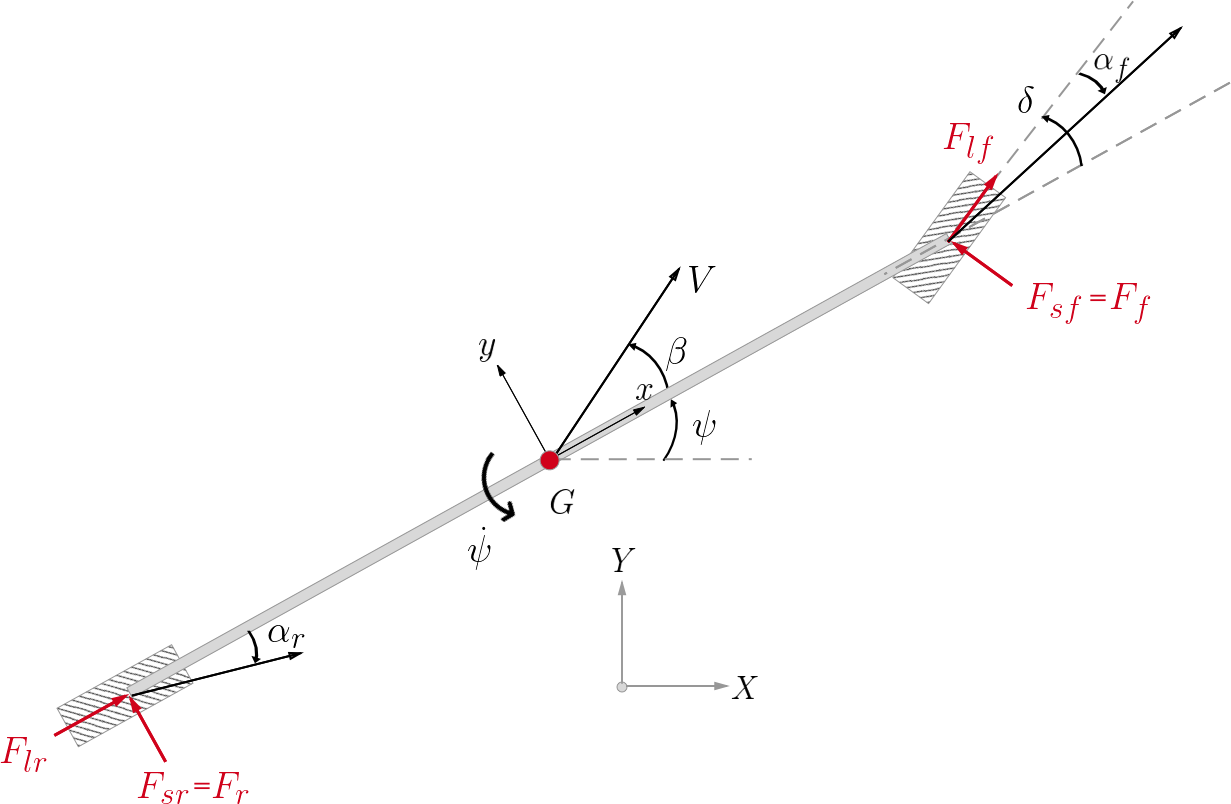
\includegraphics[width=1.0\linewidth]{figs/02/xy1}
	\caption{Bicycle model: View of the plane $XY$}
	\label{xy}
\end{figure*}

The vehicle has 3 degrees of freedom (listed below) and takes into account the effects of trail, slip angles and gyroscopic effects.

$y$ \quad Lateral position with respect to road reference \\
$\psi$ \quad Yaw angle \\ 
$\theta$ \quad Tilt angle \\
%$\delta$ \quad Front wheel steering angle 
\subsection{Model Equations}
The equations of the model implemented in this thesis have been derived using one principle:

\begin{itemize}
	\begin{itemize}
	\item The \textbf{fundamental principle of dynamics in translation and rotation}, also called Newton's laws, which require knowledge of the mechanical connections of all internal and external forces acting on the vehicle, and their points of application:
	\[\sum_{i} F=ma,\quad \sum_{j} M=I\ddot{\theta}\]
	Where $F$ represents the external forces applied to the body, $i$ the number of these forces, $m$ its mass and $a$ its acceleration. $M$ the external moments applied to the body, $j$ the number of these moments, $I$ its inertia, and $\ddot{\theta}$ its angular acceleration.
%\item The \textbf{principle of the least action and the Lagrange formalism} based on the calculation of the kinetic energy $T$ and potential $V$:
%	\[L=T-V,\quad \frac{d}{dt}\frac{\partial L}{\partial \dot{q_{i}}}-\frac{\partial L}{\partial q_{i}}=F_{q_{i}}\]
%	Where $q_{i}$ are the generalized coordinates.
	\end{itemize}
\end{itemize}
\begin{figure}
	\centering
	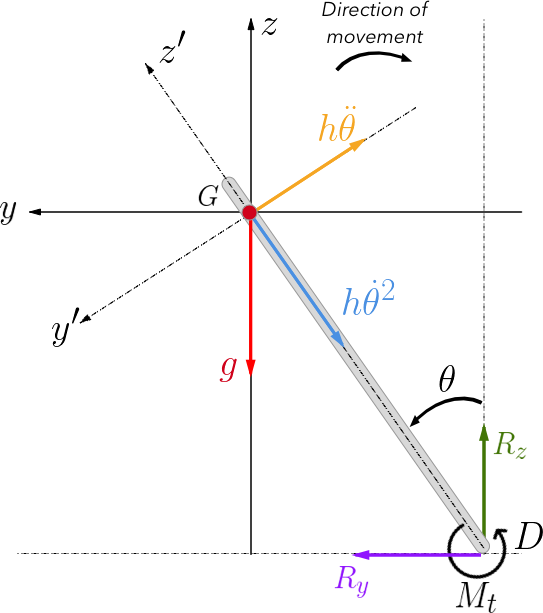
\includegraphics[width=0.85\linewidth]{figs/02/yz2}
	\caption{Bicycle model: View of the plane $YZ$}
	\label{yz}
\end{figure}
Applying Newton's principle to the presented bicycle model:\\
\minipage{0.5\textwidth}
	\[\sum_{i} \vec{F}=m\vec{a}\]
\endminipage\hfill
\minipage{0.5\textwidth}
	\begin{eqnarray}
	y) \quad R_{y}=m\,a_{y} \\
	z) \quad R_{z}-mg=m\,a_{z}
	\end{eqnarray}
\endminipage\hfill
\minipage{0.5\textwidth}
	\[\sum_{j} \vec{M}=I\vec{\ddot{\theta}}\]
\endminipage\hfill
\minipage{0.5\textwidth}
	\begin{eqnarray}
	x) \quad I_{x} \ddot{\theta}=R_{z}\,h\,\sin {\theta}\,-\,R_{y}\,h\,\cos {\theta} \\
	z) \quad I_{z} \ddot{\psi}=F_{f}\,L_{f}-F_{r}\,L_{r}
	\end{eqnarray}
\endminipage\hfill

The absolute acceleration (in the inertial reference frame $R$) of a moving body can be decoupled in two terms if a non-inertial frame of reference $r$ is attached to the body. 

Hence, the accelerations $a_{y}$ and $a_{z}$ can be obtained from the acceleration of the point $D$ (in contact with the ground), plus the relative accelerations of the center of gravity $G$ with respect to the point $D$:
\begin{eqnarray}
a_{y}=a_{D,y}+a_{G/D,y}\\
a_{z}=a_{D,z}+a_{G/D,z}
\end{eqnarray}
The center of gravity $G$ describes a circular arc of center $D$ at speed $v_{G}=h\dot{\theta}$ with $\bar{DG}=h$. The accelerations experienced at G are the tangential acceleration $\frac{dv_{G}}{dt}=h\ddot{\theta}$ along the axis $y'$, and the normal acceleration $-h\dot{\theta}^2$ along the axis $z'$.
By projecting these equations on the axes of the reference $r$=($x$, $y$, $z$):
\[a_{D,y}=\ddot{y}+V \dot{\psi}\]
\[a_{D,z}=0\]
\begin{marginfigure}[-3cm]
	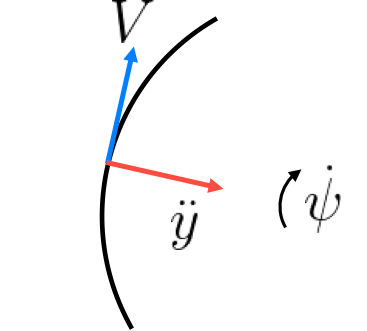
\includegraphics[width=0.8\linewidth]{figs/02/circular}
	\caption{Circular path velocity and lateral acceleration}
\end{marginfigure}

\newpage
If $D$ is taken into account as a fixed point, the relative motion can be considered:
\[v_{G}=v_{D}+\vec{w} \wedge \vec{DG}=0 + \dot{\theta}\,h(\cos {\theta}\,\vec{j}-\sin {\theta}\,\vec{k})\]
\[a_{G}=a_{D}+\vec{\alpha}\wedge\vec{DG}-w^2\,\vec{DG}=0 + \ddot{\theta}h(\cos {\theta}\,\vec{j}-\sin {\theta}\,\vec{k})-\theta^2 h (\sin {\theta}\,\vec{j}-\cos {\theta}\,\vec{k})\]
\[a_{G/D,y}=\ddot{\theta}h \cos {\theta} - \theta^2 h \sin \theta\]
\[a_{G/D,z}=-\ddot{\theta}h \sin {\theta} - \theta^2 h \cos \theta\]
Having studied the relative motion, the absolute accelerations are expressed as:
\begin{eqnarray}
a_{y}=a_{D,y}+a_{G/D,y}=\ddot{y}+V \dot{\psi}+\ddot{\theta}h \cos {\theta} - \theta^2 h \sin \theta \\
a_{z}=a_{D,z}+a_{G/D,z}=-\ddot{\theta}h \sin {\theta} - \theta^2 h \cos \theta
\end{eqnarray}
Therefore, replacing these expressions into equations (1), (2) and (3):
\[R_{y}=m\,a_{y}=m(\ddot{y}+V \dot{\psi}+\ddot{\theta}h \cos {\theta} - \theta^2 h \sin \theta)\]
\[R_{z}=m\,(a_{z}+g)=m(-\ddot{\theta}h \sin {\theta} - \theta^2 h \cos \theta + g)\]
\[I_{x} \ddot{\theta}=mh(-\ddot{\theta}h \sin^2 {\theta} - \theta^2 h \sin \theta \cos \theta + g \sin \theta -\ddot{y}\cos \theta-V \dot{\psi}\cos \theta-\ddot{\theta}h \cos^2 {\theta} + \theta^2 h \sin \theta \cos \theta)\]

The last equation represents the roll motion, and since it is going to be actuated by the motor, the tilting torque $\textcolor{blue}{M_{t}}$ has been included.
\[I_{x} \ddot{\theta}=mh(-\ddot{\theta}h + g \sin \theta -\ddot{y}\cos \theta-V \dot{\psi}\cos \theta) \textcolor{blue}{+M_{t}}\]
To get equation (4), the moment equilibrium is calculated in the c.g. Figure \ref{yaw} illustrates the vehicle from the top view, with the lateral tire forces $F_{f}$ and $F_{r}$.
\begin{equation}
I_{z} \ddot{\psi}=F_{f}\,L_{f} - F_{r}\,L_{r}
\end{equation}
\begin{marginfigure}[-5cm]
	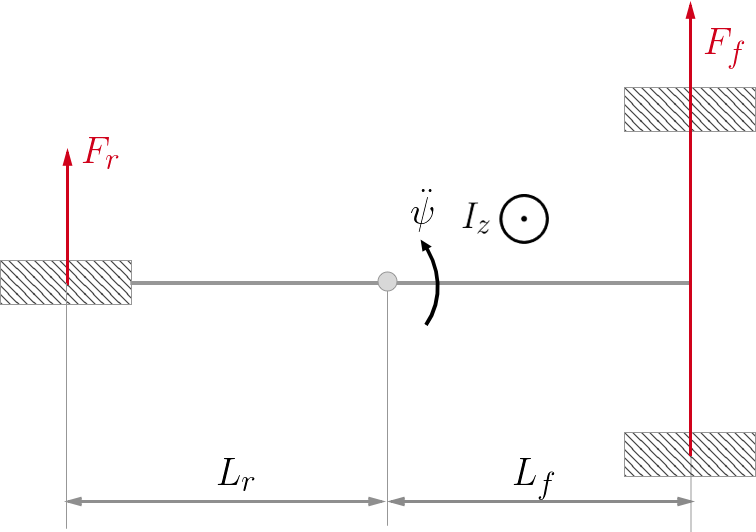
\includegraphics[width=1.2\linewidth]{figs/02/top}
	\caption{Lateral tire forces and yaw dynamics}
	\label{yaw}
\end{marginfigure}
The lateral force exerted on a wheel is expressed as $F=C\alpha + \lambda\theta$, where $C$ is the coefficient of stiffness and $\lambda\theta$ is due to the camber. Using the equality $\alpha=\delta-\tan^{-1}\Big(V_{y}/V_{x}\Big)$, at the level of the front wheels, the lateral tire forces are defined as follow for small slip angles:
\begin{eqnarray}
F_{f}=2 C_{f}\Big(\delta - \frac{\dot{y}+L_{f} \dot{\psi}}{V} \Big) + 2 \lambda_{f} \theta \\
F_{r}=C_{r}\Big(- \frac{\dot{y}-L_{r} \dot{\psi}}{V} \Big) +\lambda_{r} \theta
\end{eqnarray}
where $C_{f}$ and $C_{r}$ are the cornering stiffness of the front and rear tires, and $\lambda_{f}$ and $\lambda_{r}$ the camber stiffness of each wheel. 

\newpage
\subsubsection{\textbf{Front Wheel Dynamics due to Trail}}

The axis of the wheel has so far been considered perpendicular to the plane of the ground. This is not really the case in practice, since the axis is generally slightly inclined as shown in Figure \ref{wheels}. 
\begin{marginfigure}
	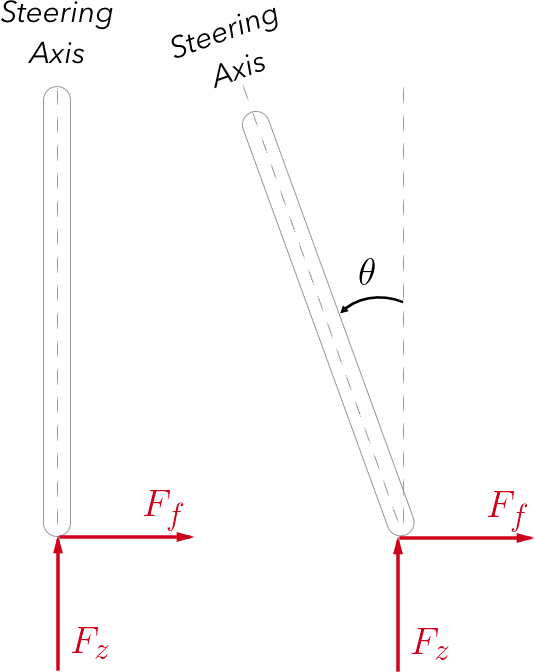
\includegraphics[width=1.0\linewidth]{figs/02/wheels}
	\caption{Inclined steering axis due to the tilting}
	\label{wheels}
\end{marginfigure}
\begin{marginfigure}
	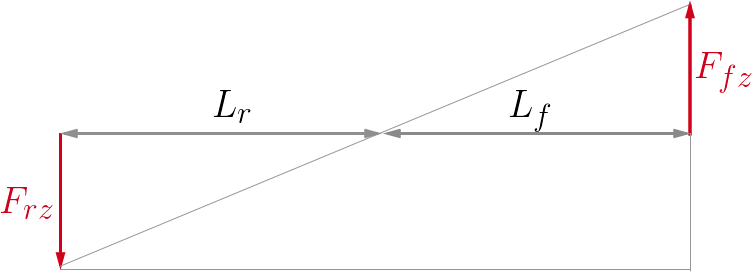
\includegraphics[width=1.2\linewidth]{figs/02/forces}
	\caption{Vertical forces diagram}
	\label{forces}
\end{marginfigure}
In absence of suspension dynamics, tilt dynamics and longitudinal acceleration, the sum of the normal forces will equal the weight of the vehicle. In addition, considering the similarity relation from Figure \ref{forces}, the normal force acting on the front wheels $F_{z}$ can be obtained:
\[\frac{F_{rz}+F_{fz}}{L_{r}+L_{f}}=\frac{F_{rz}}{L_{r}}=\frac{F_{fz}}{L_{f}}\]
\begin{equation}
F_{fz}+F_{rz}=mg \quad \Rightarrow \quad F_{fz}= F_{z}=mg \frac{L_{r}}{L_{r}+L_{f}}
\end{equation}
Thus, the reaction of the ground $F_{z}$, perpendicular to the plane of the ground, will contribute with a moment equal to $F_{z}\sin\theta$ to the steering axis. Similarly, the lateral force also contributes a restoring steering torque on the wheel (Figure \ref{trail_2}):
\begin{equation}
M_{trail}=F_{z}\gamma\cos\beta\sin\theta-F_{f}\cos\theta(\gamma+\gamma_{pneumatic})\cos\beta
\end{equation}
%\begin{marginfigure}
%	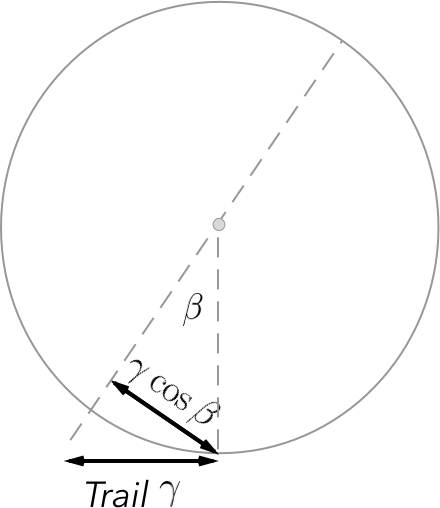
\includegraphics[width=1.1\linewidth]{figs/02/trail_1}
%	\caption{Front wheel trail}
%	\label{trail_1}
%\end{marginfigure}

\begin{figure}
	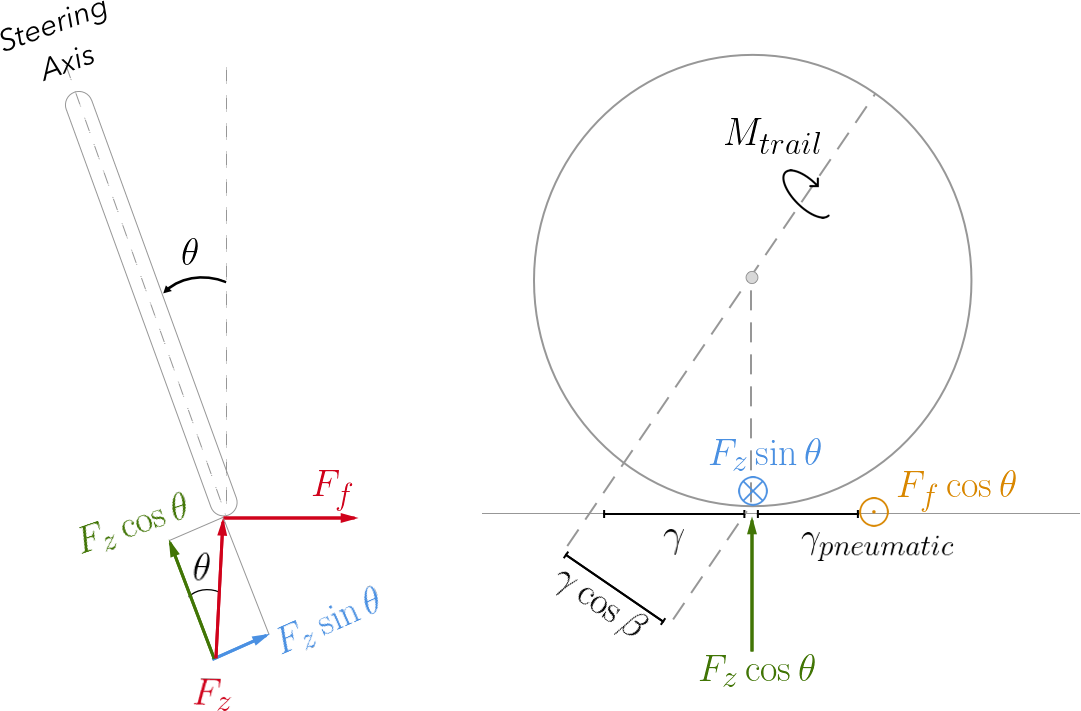
\includegraphics[width=1.1\linewidth]{figs/02/trail_2}
	\caption{Forces on front wheels when the vehicle is tilted to the left}
	\label{trail_2}
\end{figure}


\marginnote[-2.5cm]{Please notice, that the lateral force $F_f$ is not located exactly in the contact point with the ground, there exists a distance $\gamma_{pneumatic}$.}

\subsubsection{\textbf{Gyroscopic Moments}}

The dynamic equations of a rigid body with 3 rotational degrees of freedom are derived from the Euler equations:
\marginnote{Inertial reference frame:
\[\sum \vec{M}=\frac{d\vec{H}}{dt}=\frac{d(I\vec{w})}{dt} \]}
\marginnote{Non-inertial reference frame:
\[\sum \vec{M}=\Big(\frac{d(I\vec{w})}{dt}\Big)_{fixed} + \vec{w}\wedge(I\vec{w})\]}
\begin{eqnarray}
x) \quad \sum \vec{M_{x}}=I_{xx}\,\dot{\vec{w_{x}}} - (I_{yy}-I_{zz})\vec{w_{y}}\vec{w_{z}}\\
y) \quad \sum \vec{M_{y}}=I_{yy}\,\dot{\vec{w_{y}}} - (I_{zz}-I_{xx})\vec{w_{x}}\vec{w_{z}}\\
z) \quad \sum \vec{M_{z}}=I_{zz}\,\dot{\vec{w_{z}}} - (I_{xx}-I_{yy})\vec{w_{x}}\vec{w_{y}}
\end{eqnarray}

\newpage
The vehicle has two rotational degrees of freedom: yaw and roll (pitch is neglected). In addition, each rotating wheel has three rotational degrees of freedom, and Euler's equations should be applied to the rotating wheels.

Free body diagrams of the front wheels, rear wheel and vehicle body are shown in Figure \ref{body_1}. 

\begin{marginfigure}[-0.5pt]
	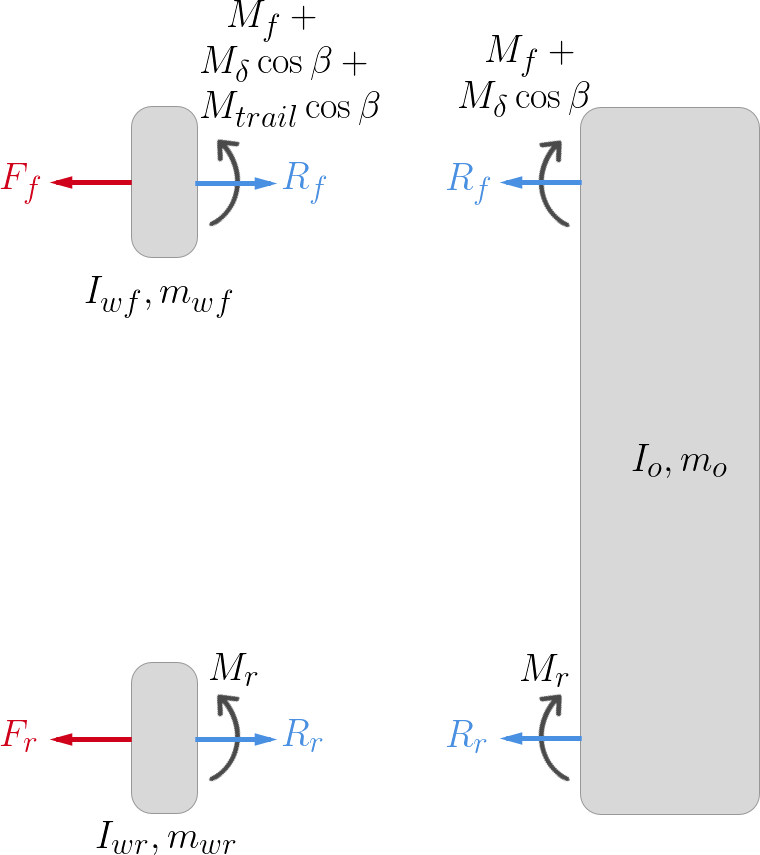
\includegraphics[width=1.3\linewidth]{figs/02/body_1}
	\caption{Free body diagram of front wheels, rear wheels and body}
	\label{body_1}
\end{marginfigure}
- \underline{Front Wheels}
\begin{eqnarray}
F_{y}) \quad 2\,m_{wf}\big(\ddot{y}+V\dot{\psi}+h_{f}\n\ddot{\theta}\cos\theta-h_{f}\dot{\theta}^2\sin\theta+L_{f}\ddot{\psi}\big)=F_{f}-R_{f} \\
M_{z}) \quad 2\,I_{wf,\psi}(\ddot{\psi}+\ddot{\delta}\cos\beta)+2(I_{wf,\theta}-I_{wf,rot})w_{rot}(\dot{\theta}-\dot{\delta}\sin\beta)=\notag\\
\quad\quad M_{f}+M_{\delta}\cos\beta+M_{trail}\cos\beta
\end{eqnarray}

- \underline{Rear Wheels}
\begin{eqnarray}
F_{y}) \quad m_{wr}\big(\ddot{y}+V\dot{\psi}+h_{r}\n\ddot{\theta}\cos\theta-h_{r}\dot{\theta}^2\sin\theta-L_{r}\ddot{\psi}\big)=F_{r}-R_{r} \\
M_{z}) \quad I_{wr,\psi}\ddot{\psi}+(I_{wr,\theta}-I_{wr,rot})w_{rot}\dot{\theta}=M_{r}
\end{eqnarray}

- \underline{Body}
\[F_{y}) \quad m_{o}\big(\ddot{y}+V\dot{\psi}+h_{o}\n\ddot{\theta}\cos\theta-h_{o}\dot{\theta}^2\sin\theta+l\ddot{\psi}\big)=R_{f}+R_{r}\]
Replacing $R_f$ and $R_r$ from front and rear wheels equations (17) and (19) onto the latter:\\[8pt]
\begin{aligned}
m_{o}\big(\ddot{y}+V\dot{\psi}+h_{o}\n\ddot{\theta}\cos\theta-h_{o}\dot{\theta}^2\sin\theta+l\ddot{\psi}\big)=\\
F_{f}-2\,m_{wf}\big(\ddot{y}+V\dot{\psi}+h_{f}\n\ddot{\theta}\cos\theta-h_{f}\dot{\theta}^2\sin\theta+L_{f}\ddot{\psi}\big) + \\
F_{r}-m_{wr}\big(\ddot{y}+V\dot{\psi}+h_{r}\n\ddot{\theta}\cos\theta-h_{r}\dot{\theta}^2\sin\theta-L_{r}\ddot{\psi}\big)
\end{aligned}

From the center of gravity property, some relations can be extracted:
\begin{itemize}[noitemsep]
\begin{itemize}[topsep=6pt]
	\item Longitudinal center of gravity: \[2\,m_{wf}\,L_{f}+m_{o}\,l-m_{wr}\,L_{r}=0 \quad \Rightarrow \quad l=\frac{m_{wr}\,L_{r}-2\,m_{wf}\,L_{f}}{m_{o}}\]
	\item Vertical center of gravity: \[m\,h=m_{o}\,h{o}+2\,m_{wf}\,h_{f}+m_{wr}\,h_{r}\]
\end{itemize}
\end{itemize}
\begin{marginfigure}[-1.5cm]
	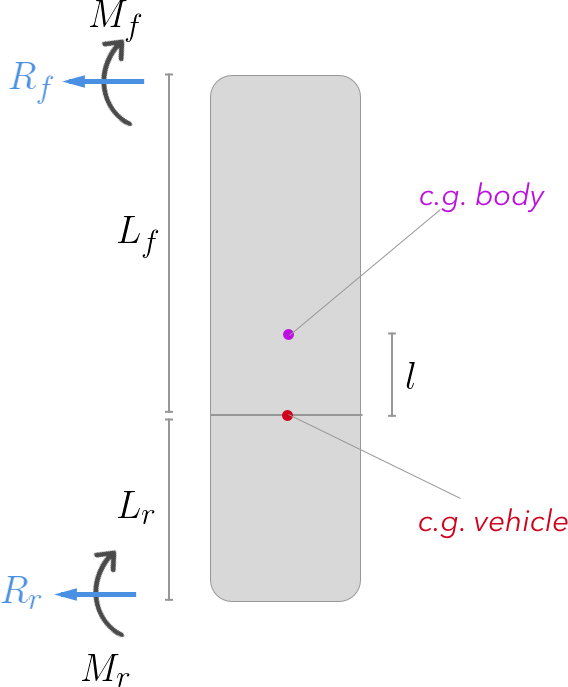
\includegraphics[width=1.1\linewidth]{figs/02/body_2}
	\caption{Free body diagram of the vehicle body}
	\label{body_1}
\end{marginfigure}
Using the relations derived above (from c.g) and simplifying:
\begin{equation}
m(\ddot{y}+V \dot{\psi}+\ddot{\theta}h \cos {\theta} - \theta^2 h \sin \theta)=F_{f}+F_{r}\]
\end{equation}
\begin{aligned}
M_{z}) \quad I_{o}\,\ddot{\psi}&=-M_{f}-M{\delta}\cos\beta-M_{r}+(L_{f}-l)R_{f}-(L_{r}+l)R_{r}\\
&=-M_{\delta}\cos\beta-2\,I_{wf,\psi}\ddot{\psi}-I_{wr,\psi}\ddot{\psi}-(I_{wr,\theta}-I_{wr,rot}w_{rot}\dot{\theta}+\\
&\quad +(L_{f}-l)\Big(F_{f}-2\,m_{wf}\big(\ddot{y}+V\dot{\psi}+h_{f}\n\ddot{\theta}\cos\theta-h_{f}\dot{\theta}^2\sin\theta+L_{f}\ddot{\psi}\big)\Big)-\\
&\quad-(L_{r}+l)\Big(F_{r}-m_{wr}\big(\ddot{y}+V\dot{\psi}+h_{r}\n\ddot{\theta}\cos\theta-h_{r}\dot{\theta}^2\sin\theta-L_{r}\ddot{\psi}\big)\Big)
\end{aligned}
\newpage
By means of the relations derived above and simplifying, the yaw dynamics equation is obtained:
\begin{equation}
I_{z}\,\ddot{\psi}=-(I_{wr,\theta}-I_{wr,rot})w_{rot}\dot{\theta}-M_{\delta}\cos\delta+L_{f}F_{f}-L_{r}L_{r}
\end{equation}
\begin{marginfigure}[-1cm]
	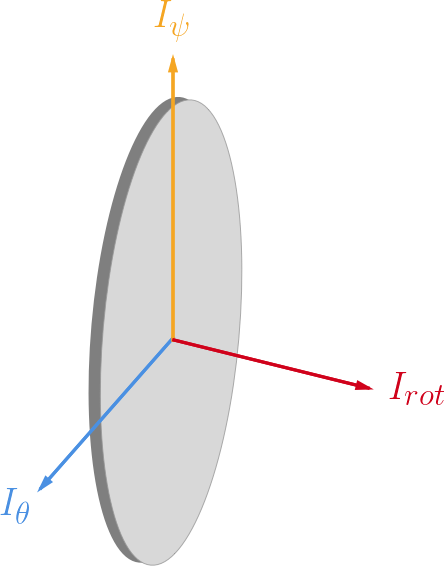
\includegraphics[width=0.9\linewidth]{figs/02/inertia}
	\caption{Front wheels axes and inertia notation}
	\label{body_1}
\end{marginfigure}
Thus the yaw dynamics have changed due to the gyroscopic terms from the rear wheel and the steering torque from the front wheels. The gyroscopic terms due to the front wheels do not appear directly in the vehicle yaw dynamic equations. Following the same procedure, the contribution to the tilt equations can be similarly derived.
\begin{itemize}
\begin{itemize}
\item With gyroscopic moments:\\$I_{z}\,\ddot{\psi}=-(I_{wr,\theta}-I_{wr,rot})w_{rot}\dot{\theta}-M_{\delta}\cos\delta+L_{f}F_{f}-L_{r}L_{r}$
\item Without gyroscopic moments: $I_{z}\,\ddot{\psi}=L_{f}F_{f}-L_{r}L_{r}$
\end{itemize}
\end{itemize}

\subsubsection{\textbf{Final Equations of Motion}}
\begin{eqnarray}
m\ddot{y}+mV \dot{\psi}+mh\ddot{\theta}\cos\theta - mh\theta^2\sin\theta=F_{f}+F_{r} \\
I_{z}\,\ddot{\psi}=L_{f}F_{f}-L_{r}L_{r}-(I_{wr,\theta}-I_{wr,rot})w_{rot}\dot{\theta}-M_{\delta}\cos\delta\\
I_{x} \ddot{\theta}=mgh\sin\theta - mh^2\ddot{\theta}\sin^2\theta - mh^2\dot{\theta}^2\cos\theta\sin\theta -\notag\\
-F_{f}h\cos\theta-F_{r}h\cos\theta +\textcolor{red}{2(I_{wf,\psi}-I_{wf,rot})w_{rot}(\dot{\psi}+\dot{\delta}\cos\beta)} + \textcolor{blue}{M_{t}}\\
2\,I_{wf,\psi}\ddot{\delta}=(M_{\delta}+M_{trail})\cos\beta-2(I_{wf,\theta}-I_{wf,rot})w_{rot}(\dot{\theta}-\dot{\delta}\sin\beta)
\end{eqnarray}

The part emphasized in red corresponds to the contribution of the gyroscopic terms to the tilting, whereas the blue part is the torque provided by the tilting motor.

\subsubsection{\textbf{Linearized Equations of Motion}}

The linearization is punctual, around the $\theta=0$ point. The longitudinal velocity is assumed constant, ($V_{x} = 8 m/s$), which is one of the most constraining hypotheses, and the angle of inclination is assumed to remain close to 0. To validate the use of this simplified model (dynamic simplifications and linearization), several velocities will be considered and the model will be linearized around several values.

The linearized equations using small angle approximations:
\begin{eqnarray}
m\ddot{y}+mV \dot{\psi}+mh\ddot{\theta}=F_{f}+F_{r} \\
I_{z}\,\ddot{\psi}=L_{f}F_{f}-L_{r}L_{r}-(I_{wr,\theta}-I_{wr,rot})w_{rot}\dot{\theta}-M_{\delta}\\
I_{x} \ddot{\theta}=mgh\theta -F_{f}h-F_{r}h + +2(I_{wf,\psi}-I_{wf,rot})w_{rot}(\dot{\psi}+\dot{\delta}) +M_{t}\\
2\,I_{wf,\psi}\ddot{\delta}=M_{\delta}+M_{trail}-2(I_{wf,\theta}-I_{wf,rot})w_{rot}\dot{\theta}
\end{eqnarray}
\newpage
\subsubsection{\textbf{Simplifying Hypotheses}}

The major simplifying hypotheses which led to the production of this bicycle model, which will serve as a support for the synthesis of control laws, are listed below: 
\begin{enumerate}\itemsep -7pt
\item Only 3 degrees of freedom: the lateral position $y$, and the tilt and yaw angles $\theta$,$\psi$. %and the steering angle $\delta$.
\item The longitudinal velocity $V_{x}$ is considered as an exogenous signal and not a system state variable. The model (2.22) is Linear Time-Variant (LTV), $V_{x}$ being a variant parameter.
\item The linearization is obtained around the angle of inclination $\theta=0$.
\item The vertical forces are assumed to be equal on both front wheels. 
\item The stiffness (slip coefficient) $C_{f}$ and the camber coefficient $\lambda_{f}$ are assumed to be constant.
\item The effect of the suspensions is neglected 
\item The wheels and the chassis are considered to be inclined to the same angle, and the point of contact of the tires do not change position during tilting.
\item The different mechanical parts moving within the vehicle, suspensions, links between different mechanical parts are not modeled.
\item The vehicle is assimilated to a mass located at the center of gravity which moves with the point of contact.
\end{enumerate}

\section{Literature Summary}

To sum up, in this chapter the literature regarding tilting vehicles has been reviewed. First, the  difference between active and passive systems was introduced, along with some examples of narrow three wheeler vehicles available to this day. In the field of active tilting systems, the distinction between the main control strategies was explained (DTC, STC and SDTC). Finally, using the literature, a dynamic model of the vehicle was derived.

The obtained linearized model is going to be the point of departure in the next chapter, regarding the control strategy.



